\tikzset{%
  every neuron/.style={
    circle,
    draw,thick,
    minimum size=0.5cm
  },
  neuron missing/.style={
    draw=none, 
    scale=4,
    text height=0.333cm,
    execute at begin node=\color{white}%$\vdots$
  },
}

\begin{figure}
    \footnotesize
    \centering
    % caption for whole f
    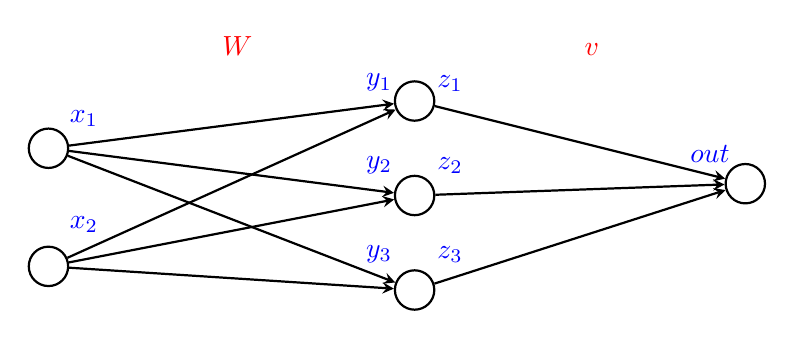
\begin{tikzpicture}[x=1.5cm, y=1.5cm, >=stealth]

        \foreach \m/\l [count=\y] in {1,2}
          \node [every neuron/.try, neuron \m/.try] (input-\m) at (-0.1,2.6-\y) {};
        
        \foreach \m [count=\y] in {1,2,3}
          \node [every neuron/.try, neuron \m/.try ] (hidden1-\m) at (3,2.8-\y*0.8) {};
        
        \foreach \m [count=\y] in {1}
          \node [every neuron/.try, neuron \m/.try ] (output-\m) at (5.8,2.3-\y) {};
        
        %\foreach \l [count=\i] in {1,2} 
        %  \draw [<-,thick] (input-\i) -- ++(-0.7,0)
         %   node [above, midway] {\scriptsize$x_\l$};
        
        %\draw [->,thick] (output-1) -- ++(0.7,0)
        %    node [above, midway] {\scriptsize$y$};

        \foreach \i in {1,...,2}
          \foreach \j in {1,...,3}
            \draw [->,thick] (input-\i) -- (hidden1-\j);

        \foreach \j in {1,...,3}
            \draw [->,thick] (hidden1-\j) -- (output-1);

       % \draw [->,thick] (input-1) -- (hidden1-1)
       %   node [above, midway] {\scriptsize$l_{21} = 1 - x_1~~$};
        %\draw [->,thick] (input-1) -- (hidden1-2)
        %  node [above, midway] {\scriptsize$l_{11} = x_1$};
        %\draw [->,thick] (input-2) -- (hidden1-3)
        %  node [above, midway] {\scriptsize$l_{12} = 1 - x_2$};
     %   \draw [->,thick] (input-2) -- (hidden1-4)
     %     node [above, midway] {\scriptsize$~~l_{22} = x_2$};
     %   \draw [->,thick] (input-3) -- (hidden1-5)
     %     node [above, midway] {\scriptsize$l_{13} = x_3$};
     %   \draw [->,thick] (input-4) -- (hidden1-6)
     %     node [above, midway] {\scriptsize$l_{23} = x_4$};
        
     %   \foreach \i in {1,4,6}
     %     \draw [->,thick] (hidden1-\i) -- (hidden2-2);

     %   \foreach \i in {2,3,5}
     %     \draw [->,thick] (hidden1-\i) -- (hidden2-1);
        %\foreach \l [count=\i] in {1,n}
        %  \node [above] at (hidden-\i.north) {$H_\l$};
        
        %\foreach \l [count=\i] in {1,n}
        %  \draw [->,thick] (output-\i) -- ++(1,0)
        %    node [above, midway] {$O_\l$};
        
        %\foreach \i in {1,...,4}
        %  \foreach \j in {1,...,2}
        %    \draw [->,thick] (input-\i) -- (hidden1-\j);
        
      %  \foreach \i in {1,...,2}
      %    \foreach \j in {1,...,2}
      %      \draw [->,thick] (hidden2-\i) -- (output-1);
        
        %\foreach \l [count=\x from 1] in {Input, Hidden, Ouput}
        %  \node [align=center, above] at (1+\x*2,2.6) {$\act_\x$};

        \node [align=center, above, color=blue] at (0.2, 1.7) {$x_1$};

        \node [align=center, above, color=blue] at (0.2, 0.8) {$x_2$};

        \node [align=center, above, color=blue] at (2.7, 1.3) {$y_2$};

        \node [align=center, above, color=blue] at (2.7, 2.0) {$y_1$};

        \node [align=center, above, color=blue] at (2.7, 0.55) {$y_3$};

        \node [align=center, above, color=blue] at (3.3, 1.3) {$z_2$};

        \node [align=center, above, color=blue] at (3.3, 2.0) {$z_1$};

        \node [align=center, above, color=blue] at (3.3, 0.55) {$z_3$};

        \node [align=center, above, color=blue] at (5.5, 1.4) {$out$};

        \node [align=center, above, color=red] at (1.5, 2.3) {$W$};
        \node [align=center, above, color=red] at (4.5, 2.3) {$v$};
        \node [align=center, above, color=red] at (3, 2.3) {$\act$};
        %\node [align=center, above] at (7, 2.5) {$\act_3$};
        
        %\node [align=center, above] at (5, 1.3) {\scriptsize$c_1=\act_2(\act_1(l_{11})+\act_1(l_{12})+\act_1(l_{13}))$};
        
        %\node [align=center, below] at (5, -1.3) {\scriptsize$c_2=\act_2(\act_1(l_{21})+\act_1(l_{22})+\act_1(l_{23}))$};
        
        %\node [align=center, below] at (7, -0.2) {\scriptsize$y = \act_3(c_1+c_2)$};
        \end{tikzpicture}
        \caption{A two-layer network example: 
$f(x) = v\act(Wx+b)+c$. We use the symbol $x$ to denote the input of the network, $y$ for the input of the hidden layer, $z$ for the output of the hidden layer, and $out$ as the out symbol. The subscript denotes the component within each symbol.}\label{fig:network}
        %\vspace{-1em}
     
\end{figure}